\documentclass[12pt,a4paper]{report}

\usepackage[T1]{fontenc}
\usepackage[french]{babel}
\usepackage{lmodern}
\usepackage{geometry}
\usepackage{graphicx}
\usepackage{amsmath, amssymb}
\usepackage{hyperref}
\usepackage{fancyhdr}
\usepackage{setspace}
\usepackage{titlesec}
\usepackage{tocloft}

\geometry{margin=2.5cm}
\onehalfspacing

\pagestyle{fancy}
\fancyhf{}
\fancyhead[L]{TP GSM}
\fancyhead[R]{\leftmark}
\fancyfoot[C]{\thepage}
\renewcommand{\headrulewidth}{0.4pt}
\setlength{\headheight}{14.5pt}

\title{
    \vspace{2cm}
    \textbf{\Huge TP GSM} \\
    \vspace{0.5cm}
}
\author{
    Groupe AR-2 : Dimitri Julmy, Dylan Flotte\\
    Computer Science\\
    HES-SO Master
}
\date{\today}

\begin{document}

\maketitle
\thispagestyle{empty}
\newpage

\tableofcontents
\newpage

\chapter*{Introduction}

Le présent rapport expose les travaux réalisés dans le cadre du laboratoire "TP3 - GSM", effectué pour le module TSM - Advanced Communication Architecture. L'objectif principal de cette manipulation est de comprendre et d'implémenter les mécanismes d'authentification et de chiffrement utilisés dans les réseaux GSM, en développant un système client-serveur simulant les échanges de sécurité.

Les étapes essentielles de l'implémentation sont suivies, depuis la génération des valeurs aléatoires (RAND) jusqu'à la mise en place d'un canal de communication sécurisé. Ce travail inclut la simulation des algorithmes cryptographiques A3 et A8, respectivement utilisés pour le calcul de la réponse signée (SRES) et la génération de la clé de session (Kc). L'architecture développée permet l'authentification mutuelle entre un client mobile et un serveur réseau, suivie du transfert sécurisé de fichiers via un chiffrement par XOR.

Ce laboratoire offre une approche pratique des protocoles de sécurité des communications mobiles de deuxième génération (2G) et permet d'appréhender les fondements sur lesquels reposent les systèmes d'authentification des réseaux cellulaires modernes.

\chapter{Code Python}

\section{config.py}
\begin{verbatim}
SERVER_HOST = "127.0.0.1"
SERVER_PORT = 5000

# Clé secrète partagée (Ki)
KI = b"SuperSecretKi123"

SESSION_DURATION = 20 * 60  # 20 minutes en secondes
BUFFER_SIZE = 4096
\end{verbatim}

\section{crypto.py}
\begin{verbatim}
import os
import hashlib

# --- RAND ---
def generate_rand():
    return os.urandom(16)  # 128 bits

# --- A3 (Simulation SRES) ---
def compute_sres(rand, ki):
    data = ki + rand
    hash_value = hashlib.sha256(data).digest()
    return hash_value[:8]  # 64 bits

# --- A8 (Simulation Kc) ---
def generate_kc(rand, ki):
    data = rand + ki
    hash_value = hashlib.sha256(data).digest()
    return hash_value[:16]  # 128-bit session key

# --- XOR Encryption/Decryption ---
def xor_cipher(data, key):
    return bytes([data[i] ^ key[i % len(key)] for i in range(len(data))])
\end{verbatim}

\section{session.py}
\begin{verbatim}
import time
from config import SESSION_DURATION

class Session:
    def __init__(self, kc):
        self.kc = kc
        self.created_at = time.time()

    def is_valid(self):
        return (time.time() - self.created_at) < SESSION_DURATION
\end{verbatim}

\section{server.py}
\begin{verbatim}
import socket
import os
from crypto import generate_rand, compute_sres, generate_kc, xor_cipher
from session import Session
from config import *

def handle_client(conn):
    try:
        print("[SERVER] Client connecté")
        print("[SERVER] Début de l'authentification")

        # 1. Génération RAND
        rand = generate_rand()
        print(f"[SERVER] RAND généré: {rand.hex()[:32]} ({len(rand)} octets)")
        conn.sendall(rand)

        # 2. Réception SRES
        client_sres = conn.recv(1024)
        print(f"[SERVER] SRES reçu du client: {client_sres.hex()} ({len(client_sres)} octets)")

        # 3. Vérification
        expected_sres = compute_sres(rand, KI)
        print(f"[SERVER] SRES attendu: {expected_sres.hex()}")

        if client_sres != expected_sres:
            conn.sendall(b"AUTH_FAILED")
            print("[SERVER] Authentification échouée")
            return

        conn.sendall(b"AUTH_SUCCESS")
        print("[SERVER] Authentification réussie")

        # 4. Génération session
        kc = generate_kc(rand, KI)
        print(f"[SERVER] Clé de session Kc générée: {kc.hex()[:32]} ({len(kc)} octets)")
        session = Session(kc)
        print(f"[SERVER] Session créée à {session.created_at}")

        # 5. Réception fichier chiffré
        print("[SERVER] Réception du fichier chiffré")
        encrypted_data = b""
        chunk_count = 0
        while True:
            chunk = conn.recv(BUFFER_SIZE)
            if not chunk:
                break
            encrypted_data += chunk
            chunk_count += 1

        print(f"[SERVER] Fichier chiffré complet reçu: {len(encrypted_data)} octets")

        if not session.is_valid():
            print("[SERVER] Session expirée")
            return

        print("[SERVER] Déchiffrement en cours")
        decrypted_data = xor_cipher(encrypted_data, session.kc)
        print(f"[SERVER] Fichier déchiffré: {len(decrypted_data)} octets")

        with open("files/server_received.mp3", "wb") as f:
            f.write(decrypted_data)

        print("[SERVER] Fichier reçu et déchiffré")

        # 6. Envoi fichier serveur
        print("[SERVER] Lecture du fichier à envoyer")
        with open("files/bombinsound-rap-rap-beat-beats-music-20-second-491118.mp3", "rb") as f:
            data = f.read()

        print(f"[SERVER] Fichier lu: {len(data)} octets")
        print("[SERVER] Chiffrement en cours")
        encrypted_response = xor_cipher(data, session.kc)
        print(f"[SERVER] Fichier chiffré: {len(encrypted_response)} octets")
        print("[SERVER] Envoi du fichier")
        conn.sendall(encrypted_response)

        print("[SERVER] Fichier envoyé")

    except Exception as e:
        print(f"[SERVER ERROR] {e}")
    finally:
        conn.close()

def start_server():
    server = socket.socket(socket.AF_INET, socket.SOCK_STREAM)
    server.setsockopt(socket.SOL_SOCKET, socket.SO_REUSEADDR, 1)
    server.bind((SERVER_HOST, SERVER_PORT))
    server.listen(1)
    print(f"[SERVER] En écoute sur {SERVER_HOST}:{SERVER_PORT}")

    while True:
        conn, addr = server.accept()
        handle_client(conn)

if __name__ == "__main__":
    start_server()
\end{verbatim}

\section{client.py}
\begin{verbatim}
import socket
from crypto import compute_sres, generate_kc, xor_cipher
from config import *

def start_client():
    print(f"[CLIENT] Connexion au serveur {SERVER_HOST}:{SERVER_PORT}")
    client = socket.socket(socket.AF_INET, socket.SOCK_STREAM)
    client.connect((SERVER_HOST, SERVER_PORT))
    print("[CLIENT] Connecté")

    # 1. Réception RAND
    rand = client.recv(1024)
    print(f"[CLIENT] RAND reçu: {rand.hex()[:32]} ({len(rand)} octets)")

    # 2. Calcul SRES
    print("[CLIENT] Calcul du SRES")
    sres = compute_sres(rand, KI)
    print(f"[CLIENT] SRES calculé: {sres.hex()} ({len(sres)} octets)")
    client.sendall(sres)
    print("[CLIENT] SRES envoyé au serveur")

    # 3. Vérification résultat
    response = client.recv(1024)
    print(f"[CLIENT] Réponse d'authentification: {response.decode('utf-8', errors='ignore')}")

    if response != b"AUTH_SUCCESS":
        print("[CLIENT] Authentification échouée")
        return

    print("[CLIENT] Authentification réussie")

    # 4. Génération Kc
    print("[CLIENT] Génération de la clé de session")
    kc = generate_kc(rand, KI)
    print(f"[CLIENT] Clé de session Kc: {kc.hex()[:32]} ({len(kc)} octets)")

    # 5. Envoi fichier
    print("[CLIENT] Lecture du fichier à envoyer")
    with open("files/bombinsound-rap-rap-beat-beats-music-20-second-491118.mp3", "rb") as f:
        data = f.read()

    print(f"[CLIENT] Fichier lu: {len(data)} octets")
    print("[CLIENT] Chiffrement en cours")
    encrypted_data = xor_cipher(data, kc)
    print(f"[CLIENT] Fichier chiffré: {len(encrypted_data)} octets")
    print("[CLIENT] Envoi du fichier")
    client.sendall(encrypted_data)
    client.shutdown(socket.SHUT_WR)

    print("[CLIENT] Fichier envoyé")

    # 6. Réception fichier serveur
    print("[CLIENT] Réception du fichier du serveur")
    encrypted_response = b""
    chunk_count = 0
    while True:
        chunk = client.recv(BUFFER_SIZE)
        if not chunk:
            break
        encrypted_response += chunk
        chunk_count += 1

    print(f"[CLIENT] Fichier chiffré complet reçu: {len(encrypted_response)} octets")
    print("[CLIENT] Déchiffrement en cours")
    decrypted_response = xor_cipher(encrypted_response, kc)
    print(f"[CLIENT] Fichier déchiffré: {len(decrypted_response)} octets")

    with open("files/client_received.mp3", "wb") as f:
        f.write(decrypted_response)

    print("[CLIENT] Fichier reçu et déchiffré")

    client.close()
    print("[CLIENT] Connexion fermée")

if __name__ == "__main__":
    start_client()
\end{verbatim}

\chapter{Capture du fonctionnement}

\begin{figure}[h]
	\centering
    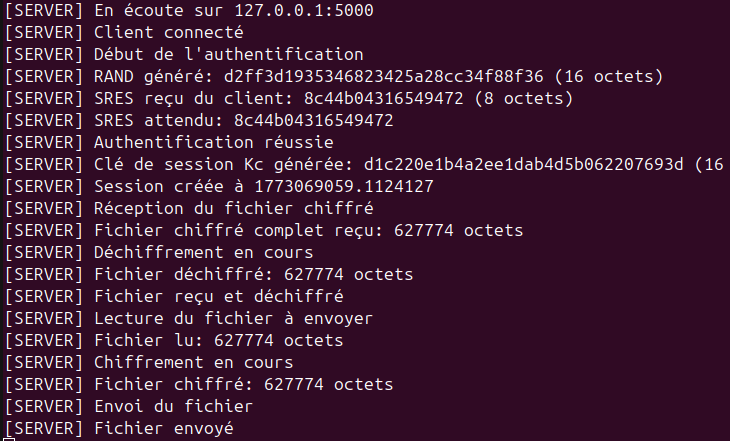
\includegraphics[width=1\textwidth]{Cap1.png}
    \caption{Capture fonctionnement côté serveur}
    \label{fig:monimage}
\end{figure}

\begin{figure}[h]
	\centering
    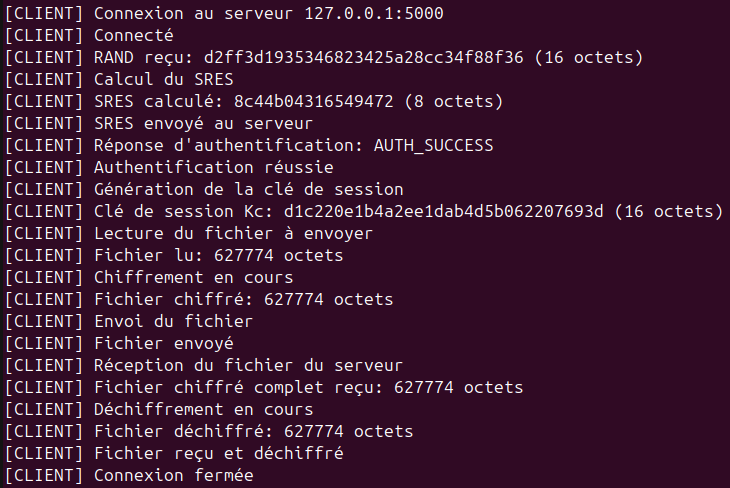
\includegraphics[width=1\textwidth]{Cap2.png}
    \caption{Capture fonctionnement côté client}
    \label{fig:monimage}
\end{figure}

\chapter*{Conclusion}

Ce laboratoire a permis de valider la mise en œuvre complète d'un système d'authentification GSM, confirmant le bon fonctionnement des algorithmes cryptographiques A3 et A8, ainsi que l'établissement d'un canal de communication sécurisé entre le client et le serveur. L'implémentation développée illustre les mécanismes fondamentaux de génération de RAND, de calcul de SRES et de dérivation de la clé de session Kc, permettant ainsi de comprendre concrètement les protocoles d'authentification des réseaux mobiles 2G.

Malgré la simplicité du chiffrement par XOR utilisé dans cette simulation, l'architecture mise en place démontre efficacement les principes de l'authentification unidirectionnelle et du transfert sécurisé de données. Les captures de fonctionnement présentées attestent de la réussite de l'échange cryptographique entre les deux entités et de la validité de la session établie.

Enfin, cette étude pratique met en perspective les limitations inhérentes aux systèmes GSM, notamment la vulnérabilité du chiffrement A5/1 et l'absence d'authentification mutuelle dans les premières versions du protocole. Elle souligne l'importance de l'évolution vers les standards 3G (UMTS) et 4G (LTE) qui ont introduit des mécanismes d'authentification bidirectionnelle et des algorithmes cryptographiques plus robustes. Cette expérience constitue ainsi une base solide pour appréhender les architectures de sécurité des communications mobiles modernes et leur évolution historique.

\end{document}
